% 1961 年全国卷第 6 题：三角形到平面的正投影。
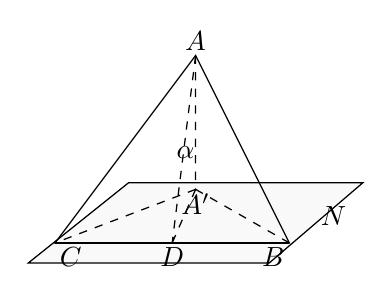
\begin{tikzpicture}[scale=0.85, line width=0.45pt,
  every node/.style={inner sep=1.5pt}]
  \coordinate (C) at (-2.0,-0.8);
  \coordinate (B) at (1.5,-0.8);
  \coordinate (A) at (0.1,2.0);
  \coordinate (Ap) at (0.1,0.0);
  \coordinate (D) at (-0.25,-0.8);
  \draw[fill=gray!5] (-2.4,-1.1)--(1.2,-1.1)--(2.6,0.1)--(-0.9,0.1)--cycle;
  \draw (A)--(B)--(C)--cycle;
  \draw[dashed] (A)--(Ap) (Ap)--(B) (Ap)--(C);
  \draw[dashed] (A)--(D) (Ap)--(D);
  \draw (C)--(B);
  \node[anchor=south] at (A) {$A$};
  \node[anchor=north] at (Ap) {$A'$};
  \node[anchor=north east] at (B) {$B$};
  \node[anchor=north west] at (C) {$C$};
  \node[anchor=north] at (D) {$D$};
  \node[anchor=west] at (1.9,-0.4) {$N$};
  \node at (-0.05,0.55) {$\alpha$};
\end{tikzpicture}
